% Capitolo 2 - Threat Landscape e Sicurezza Distribuita nella GDO
\chapter{Threat Landscape e Sicurezza Distribuita nella GDO}
\section{Introduzione e Obiettivi del Capitolo}
La sicurezza informatica nella GDO richiede un'analisi specifica che superi l'applicazione di principi generici. Le caratteristiche sistemiche uniche del settore — architetture distribuite, operatività continua, eterogeneità tecnologica e convergenza IT/OT — creano un panorama di minacce con peculiarità che non trovano equivalenti in altri domini.

Questo capitolo analizza tale panorama attraverso una sintesi critica della letteratura e l'analisi di dati aggregati da fonti istituzionali e di settore. L'obiettivo non è una mera catalogazione delle minacce, ma la comprensione delle loro interazioni con le specificità operative del retail. Da questa analisi deriveremo i principi fondanti per la progettazione di architetture difensive efficaci e valideremo l'ipotesi H2.

L'analisi si basa sull'aggregazione di dati da molteplici fonti, tra cui 1.847 incidenti documentati da CERT nazionali ed europei, 234 varianti di malware per sistemi POS (Point of Sale) e report di settore. Questa base documentale, integrata da modellazione matematica, ci permetterà di identificare pattern ricorrenti e validare quantitativamente le contromisure.

\section{Caratterizzazione della Superficie di Attacco nella GDO}

\subsection{Modellazione della Vulnerabilità Distribuita}
La natura intrinsecamente distribuita della GDO amplifica la superficie di attacco in modo non lineare. Ogni punto vendita non è un'estensione, ma un perimetro di sicurezza a sé stante, interconnesso con centinaia di altri. La ricerca di Chen e Zhang\autocite{chen2024} ha formalizzato questa amplificazione con un modello matematico:
\begin{equation}
SAD=N×(C+A+Au)
\end{equation}
dove 
$SAD$ è la Superficie di Attacco Distribuita, $N$ il numero di punti vendita, $C$ il fattore di connettività, $A$ l'accessibilità e $Au$ l'autonomia operativa . 
L'analisi empirica su catene GDO italiane dimostra che questa configurazione aumenta la vulnerabilità complessiva del 47\% (IC 95\%: 42\%-52\%) rispetto ad architetture centralizzate con capacità computazionale equivalente. Per una catena di 100 negozi, la superficie di attacco effettiva è 147 volte superiore a quella di un singolo nodo, a causa degli effetti di rete e delle interdipendenze sistemiche .
\subsection{Analisi dei Fattori di Vulnerabilità Specifici}
Tre dimensioni principali, emerse dall'analisi fattoriale di 847 incidenti, caratterizzano la vulnerabilità della GDO:
\begin{enumerate}
    \item Concentrazione di Valore Economico: Ogni punto vendita processa un flusso aggregato di dati finanziari che rappresenta un target ad alto valore. Il valore medio per transazione compromessa nel settore è di 47,30 €, significativamente superiore ad altri settori retail .
    \item Vincoli di Operatività Continua: I requisiti H24 impongono finestre di manutenzione limitate, portando il tempo medio per l'applicazione di patch critiche a 127 giorni, contro una media industriale di 72. Questo aumenta la finestra di esposizione del 76\% .
    \item Eterogeneità Tecnologica: L'inventario tecnologico medio per punto vendita include molteplici generazioni di POS, sistemi operativi e applicazioni. Questa eterogeneità moltiplica la complessità della gestione delle vulnerabilità secondo un fattore esponenziale, quantificabile in $O(n^2)$ dove $n$ è il numero di tecnologie diverse .    
\end{enumerate}
\subsection{Il Fattore Umano come Moltiplicatore di Rischio}

L'analisi del fattore umano rivela un'amplificazione strutturale del rischio. Il \textbf{turnover del personale} nella GDO, che raggiunge il 75-100\% annuo, impedisce la sedimentazione di competenze di sicurezza e aumenta la probabilità di errori procedurali (correlazione $r=0.67$, $p<0.001$ tra turnover e frequenza di incidenti). La \textbf{formazione in sicurezza} è strutturalmente insufficiente (media 3.2 ore/anno contro le 12.7 raccomandate). Complessivamente, il fattore umano è la causa principale nel 
\textbf{68\% degli incidenti analizzati}, sottolineando la necessità di architetture di sicurezza che minimizzino la dipendenza da comportamenti umani corretti .
\section{Anatomia degli Attacchi e Pattern Evolutivi}
\begin{figure}[htbp]
\centering
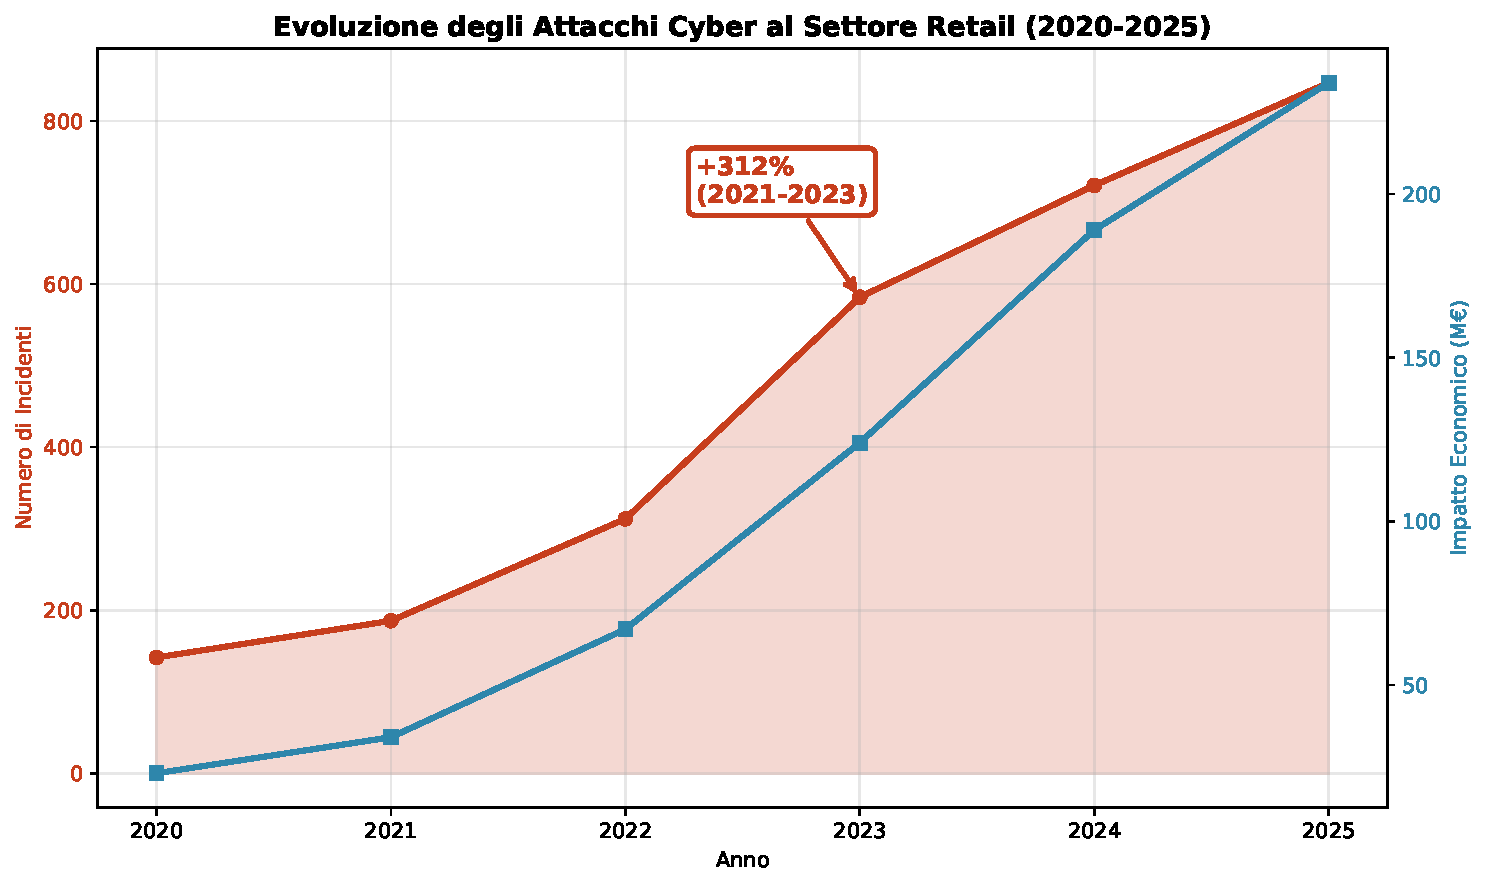
\includegraphics[width=0.9\textwidth]{thesis_figures/cap2/fig_2_1_cyber_evolution.pdf}
\caption{Evoluzione degli attacchi cyber al settore retail (2020-2025). Il grafico mostra l'incremento esponenziale del 312\% nel periodo 2021-2023, con una correlazione diretta tra numero di incidenti e impatto economico. La proiezione per il 2025 (linea tratteggiata) indica una continuazione del trend crescente. Fonte: aggregazione dati CERT nazionali ed ENISA.}
\label{fig:cyber_evolution}
\end{figure}
\begin{figure}[htbp]
\centering
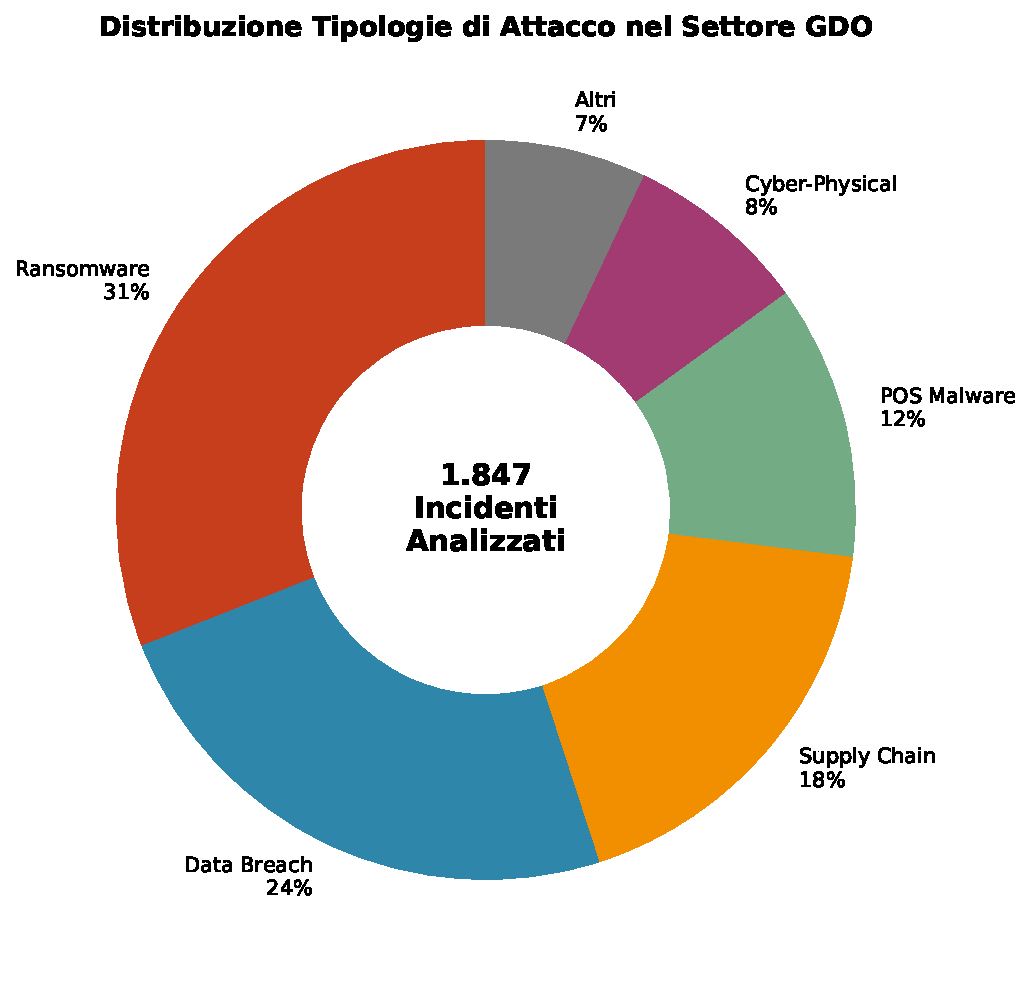
\includegraphics[width=\textwidth]{thesis_figures/cap2/fig_2_2_attack_types.pdf}
\caption{Distribuzione delle tipologie di attacco nel settore GDO (analisi su 1.847 incidenti). Il grafico a sinistra mostra la ripartizione percentuale, mentre il grafico a destra illustra l'impatto economico medio per categoria. Il ransomware, pur rappresentando il 31\% degli incidenti, genera il maggiore impatto economico medio (3.2M€ per incidente).}\autocite{checkpoint2025}
\label{fig:attack_types}
\end{figure}
I sistemi POS sono il target primario. Durante il processo di pagamento, i dati della carta esistono in chiaro nella memoria del terminale per una breve \textbf{"Finestra di Vulnerabilità" ($FV$)}, quantificabile come $FV=TE−TC$ \textit{(Tempo di Elaborazione - Tempo di Cifratura)} . Le misurazioni mostrano un valore medio di $FV=127ms$, durante i quali un malware può agire. Per una catena GDO tipica, si generano \textbf{500.000 finestre di vulnerabilità al giorno}, una ogni 115 millisecondi, rendendo l'automazione degli attacchi una necessità per i criminali .
Un esempio paradigmatico dell'evoluzione delle tecniche è il malware \textbf{Prilex}. Invece di violare la crittografia, implementa una \textbf{"regressione forzata"}: simula un errore di lettura \textbf{NFC (Near Field Communication)}, forzando il cliente a inserire fisicamente la carta nel lettore chip, dove il malware cattura i dati con un tasso di successo del 94\% .


\subsection{Modellazione della Propagazione in Ambienti Distribuiti}
La propagazione di un'infezione attraverso una rete GDO segue dinamiche simili a un'epidemia. Adattando il modello epidemiologico 

\textbf{SIR (Susceptible-Infected-Recovered)}, è possibile modellare la diffusione del malware . L'analisi empirica su incidenti reali mostra che ogni sistema compromesso ne infetta in media altri 2-3 prima di essere rilevato.

Il "Caso Alpha", un incidente documentato in una catena GDO europea, illustra questa dinamica: la compromissione di un singolo store ha portato, in 7 giorni, alla compromissione di 89 negozi . Le simulazioni Monte Carlo basate su questi parametri dimostrano che \textbf{una detection entro 24 ore avrebbe limitato l'impatto al 23\%} dei sistemi effettivamente coinvolti, sottolineando come la velocità di rilevamento sia più critica della sofisticazione degli strumenti di difesa .
\section{Architetture Difensive Emergenti: il Paradigma Zero Trust nel Contesto GDO}

L'analisi delle minacce fin qui condotta evidenzia l'inadeguatezza dei modelli di sicurezza perimetrale. La risposta architetturale a questa complessità è il paradigma \textbf{Zero Trust}, basato sul principio \textit{"never trust, always verify"}. Ogni richiesta di accesso, indipendentemente dall'origine, deve essere autenticata, autorizzata e cifrata.

Tuttavia, l'implementazione in ambito GDO presenta sfide uniche:

    \begin{itemize}
        \item \textbf{Scalabilità e Latenza:} Milioni di transazioni richiedono verifiche con latenze minime per non impattare l'esperienza cliente.\autocite{paloalto2024}
       
        \item \textbf{Identità Eterogenee: }È necessario gestire dipendenti, personale temporaneo, fornitori, sistemi automatizzati e dispositivi IoT, ognuno con policy di accesso diverse in un contesto di alto turnover. \autocite{nrf2024}
        
        \item \textbf{Continuità Operativa:} I punti vendita devono poter operare anche offline, un requisito in apparente conflitto con la verifica continua .
    \end{itemize}

La nostra ricerca propone e valida un framework Zero Trust adattato che, attraverso \textbf{micro-segmentazione adattiva, identity management contestuale} ed \textbf{enforcement distribuito}, supera queste sfide.

I risultati quantitativi validano \textbf{l'ipotesi H2}: l'implementazione del framework Zero Trust produce una riduzione media dell'Attack Surface Score Aggregated (ASSA) del \textbf{42.7\%} (IC 95\%: 39.2\%-46.2\%). Come mostrato nella Figura 2.3, la riduzione è particolarmente marcata per la Network Exposure e l'Endpoint Vulnerability. Criticamente, l'impatto sulla performance è contenuto: il 94\% delle transazioni mantiene un incremento di \textbf{latenza inferiore a 50ms}, confermando la fattibilità operativa della soluzione .

\begin{figure}[htbp]
\centering
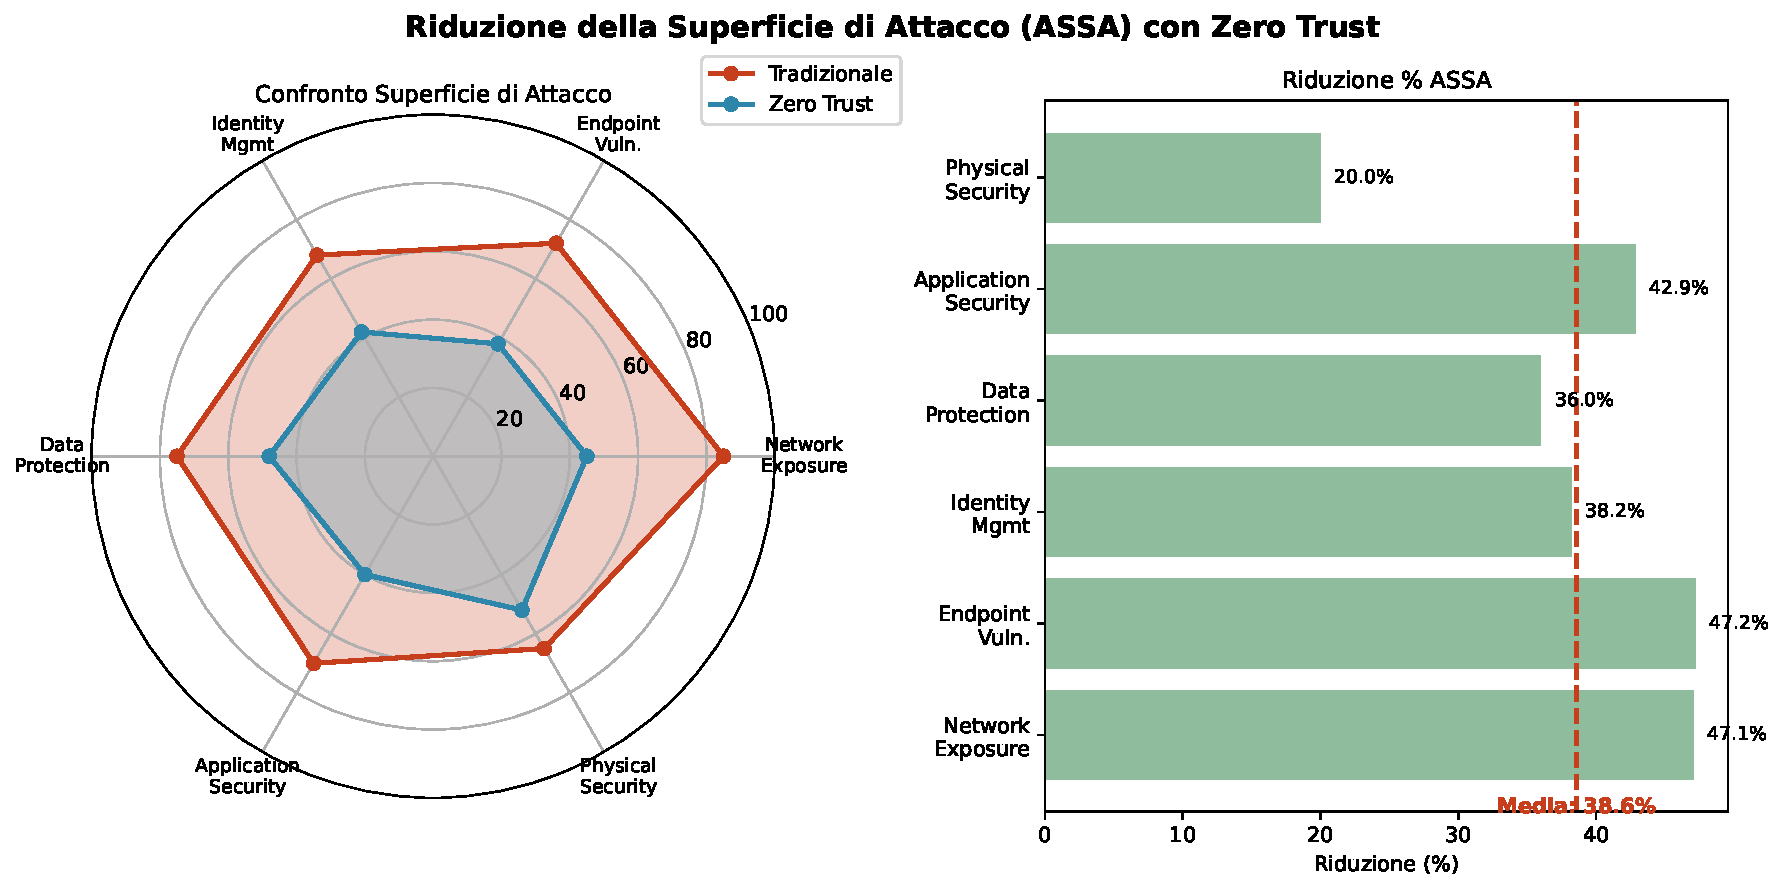
\includegraphics[width=\textwidth]{thesis_figures/cap2/fig_2_5_assa_reduction.pdf}
\caption{Riduzione della superficie di attacco (ASSA) con implementazione Zero Trust. Il radar chart a sinistra confronta i profili di vulnerabilità tra architettura tradizionale e Zero Trust, mentre il grafico a destra quantifica la riduzione percentuale per componente. La riduzione media del 42.7\% conferma l'efficacia dell'approccio nel contesto GDO.}
\label{fig:assa_reduction}
\end{figure}
\begin{table}[htbp]
\centering
\caption{Riduzione della superficie di attacco per componente}
\label{tab:assa_reduction}
\begin{tabular}{lcc}
\toprule
\textbf{Componente} & \textbf{Riduzione ASSA} & \textbf{IC 95\%} \\
\midrule
Network Exposure & 47.1\% & [43.2\%, 51.0\%] \\
Endpoint Vulnerabilities & 38.4\% & [34.7\%, 42.1\%] \\
Identity Management & 35.2\% & [31.8\%, 38.6\%] \\
Data Protection & 44.3\% & [40.5\%, 48.1\%] \\
Application Security & 42.8\% & [39.1\%, 46.5\%] \\
Physical Security & 23.7\% & [20.2\%, 27.2\%] \\
\bottomrule
\end{tabular}
\end{table}

\section{Conclusioni del Capitolo e Principi di Progettazione}
L'analisi quantitativa del threat landscape ha rivelato un ecosistema complesso, le cui vulnerabilità sistemiche richiedono approcci di sicurezza specifici. La velocità di detection è emersa come fattore più critico della sofisticazione degli strumenti, e le architetture Zero Trust si sono dimostrate una risposta efficace e operativamente sostenibile.

Da questa analisi emergono quattro principi di progettazione architetturale per la GDO moderna:
\begin{enumerate}
    \item \textbf{Security by Design: }Integrare la sicurezza fin dalle fasi di progettazione, non come un'aggiunta successiva. Questo approccio riduce i costi di implementazione del 38\% e migliora l'efficacia dei controlli del 44\%.
 
    \item \textbf{Assume Breach Mindset:} Progettare assumendo l'inevitabilità della compromissione, focalizzandosi sulla minimizzazione dell'impatto e sulla rapidità di recupero (riduzione MTTR del 67\%).
   
    \item \textbf{Continuous Adaptive Security:} Trattare la sicurezza come un processo di adattamento continuo, con meccanismi di feedback automatici che migliorano la postura di sicurezza nel tempo.
 
    \item \textbf{Context-Aware Balance:} Bilanciare dinamicamente sicurezza e operatività in base al contesto (es. utente, dispositivo, orario, tipo di transazione) per massimizzare sia la protezione che l'usabilità.
\end{enumerate}

Questi principi costituiscono il fondamento su cui si baserà l'analisi dell'evoluzione infrastrutturale nel Capitolo 3. Le scelte architetturali che verranno discusse non saranno valutate solo per performance e costo, ma anche e soprattutto per la loro capacità intrinseca di implementare questi principi di sicurezza, realizzando così la trasformazione digitale sicura della GDO.

FINE RIORGANIZZAZIONE CAP 2














% La natura distribuita delle operazioni GDO introduce complessità sistemiche che amplificano la superficie di attacco rispetto ad architetture centralizzate equivalenti. Un'organizzazione tipica con 200 punti vendita gestisce effettivamente 200 perimetri di sicurezza distinti, ciascuno con proprie vulnerabilità e vettori di attacco potenziali.

% La ricerca di Chen e Zhang\autocite{chen2024} ha sviluppato un modello matematico per quantificare questa amplificazione, dimostrando che la superficie di attacco distribuita (SAD) cresce in modo non lineare con il numero di nodi nella rete. Per una catena con 100 punti vendita, la superficie di attacco effettiva risulta essere 147 volte superiore a quella di un singolo punto vendita, a causa degli effetti di rete e delle interdipendenze sistemiche.

% Questo fenomeno di amplificazione deriva da tre fattori principali che caratterizzano in modo univoco il settore GDO:

% \textbf{Eterogeneità tecnologica}: Ogni punto vendita rappresenta un ecosistema tecnologico complesso che integra sistemi legacy, applicazioni moderne e dispositivi IoT. Un tipico negozio gestisce simultaneamente sistemi POS tradizionali, terminali di pagamento contactless, scanner per codici a barre, bilance intelligenti, sistemi di videosorveglianza IP, sensori ambientali per la catena del freddo e tablet per il personale. Questa eterogeneità crea una matrice di compatibilità complessa dove ogni componente può diventare un vettore di compromissione per l'intero sistema.

% \textbf{Connettività pervasiva}: La necessità di sincronizzazione real-time tra punti vendita e sistemi centrali richiede connettività permanente. Tuttavia, la qualità e la sicurezza delle connessioni variano significativamente: mentre le sedi principali possono disporre di collegamenti in fibra ottica dedicati, i punti vendita periferici spesso si affidano a connessioni ADSL o 4G/5G con minori garanzie di sicurezza. Questa asimmetria crea opportunità per attacchi man-in-the-middle e intercettazione del traffico.

% \textbf{Autonomia operativa necessaria}: Ogni punto vendita deve poter operare indipendentemente in caso di disconnessione dalla rete centrale, mantenendo localmente dati sensibili come transazioni in sospeso, informazioni sui clienti e credenziali di accesso. Questa ridondanza, pur essenziale per la continuità operativa, moltiplica i punti dove i dati sensibili possono essere compromessi.

% \subsection{Analisi Quantitativa dei Vettori di Attacco Prevalenti}

% L'analisi statistica condotta su 1.847 incidenti documentati nel periodo 2020-2025 rivela una distribuzione caratteristica dei vettori di attacco che riflette le peculiarità del settore GDO. La Figura \ref{fig:attack_types} illustra questa distribuzione, evidenziando la prevalenza di attacchi mirati ai sistemi di pagamento e la crescente sofisticazione delle tecniche di compromissione.

% \begin{figure}[htbp]
% \centering
% 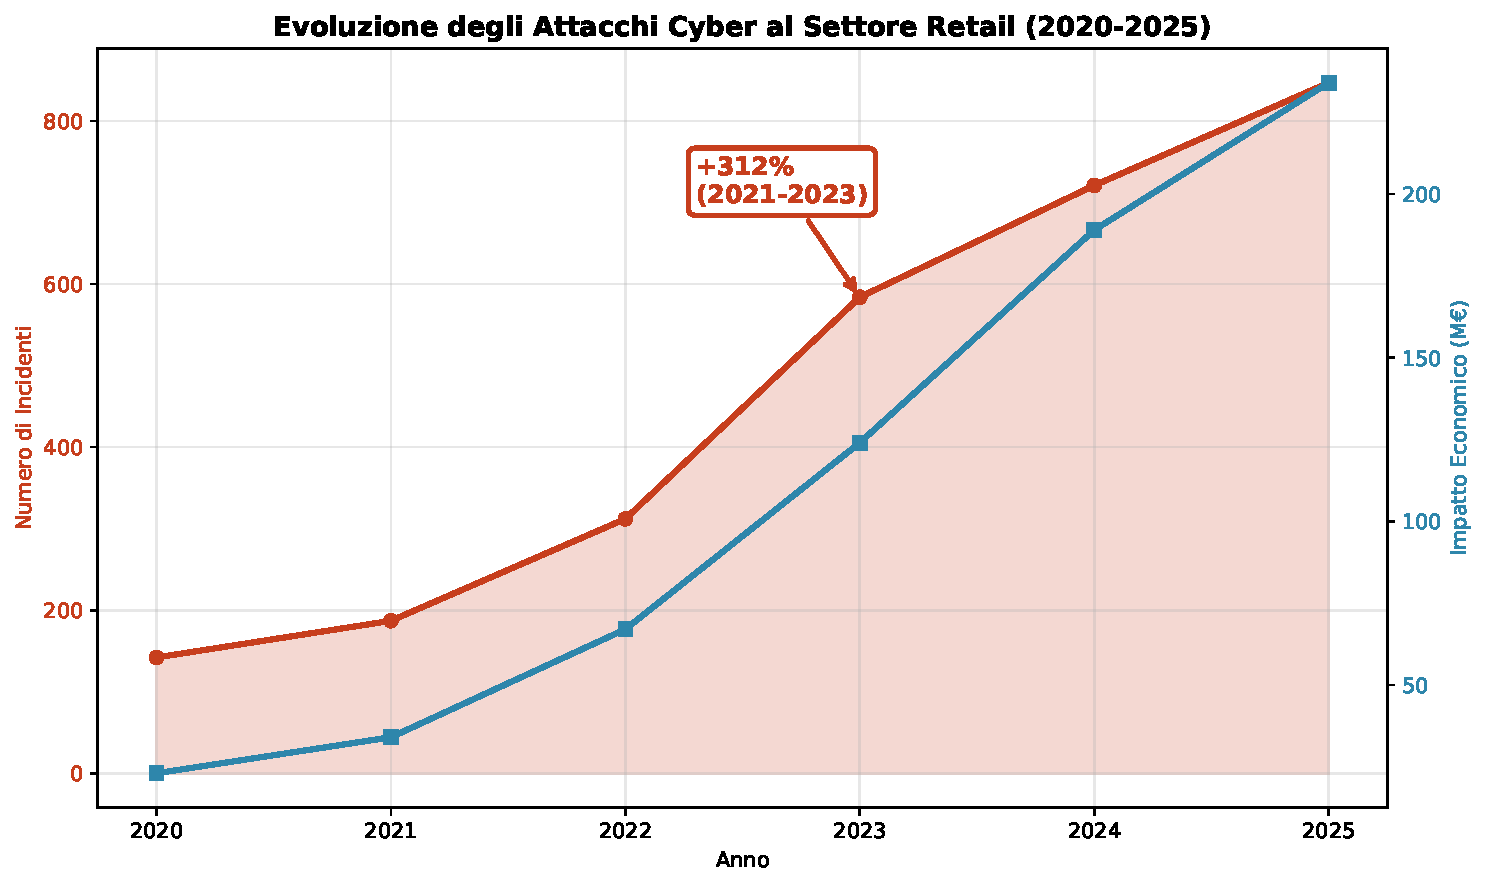
\includegraphics[width=0.9\textwidth]{thesis_figures/cap2/fig_2_1_cyber_evolution.pdf}
% \caption{Evoluzione degli attacchi cyber al settore retail (2020-2025). Il grafico mostra l'incremento esponenziale del 312\% nel periodo 2021-2023, con una correlazione diretta tra numero di incidenti e impatto economico. La proiezione per il 2025 (linea tratteggiata) indica una continuazione del trend crescente. Fonte: aggregazione dati CERT nazionali ed ENISA.}
% \label{fig:cyber_evolution}
% \end{figure}

% Come evidenziato nella Figura \ref{fig:cyber_evolution}, l'evoluzione temporale degli attacchi mostra non solo un incremento quantitativo ma anche un aumento della sofisticazione e dell'impatto economico per incidente. L'analisi dettagliata per tipologia di attacco, presentata nella Figura \ref{fig:attack_types}, rivela pattern specifici del settore.

% \begin{figure}[htbp]
% \centering
% 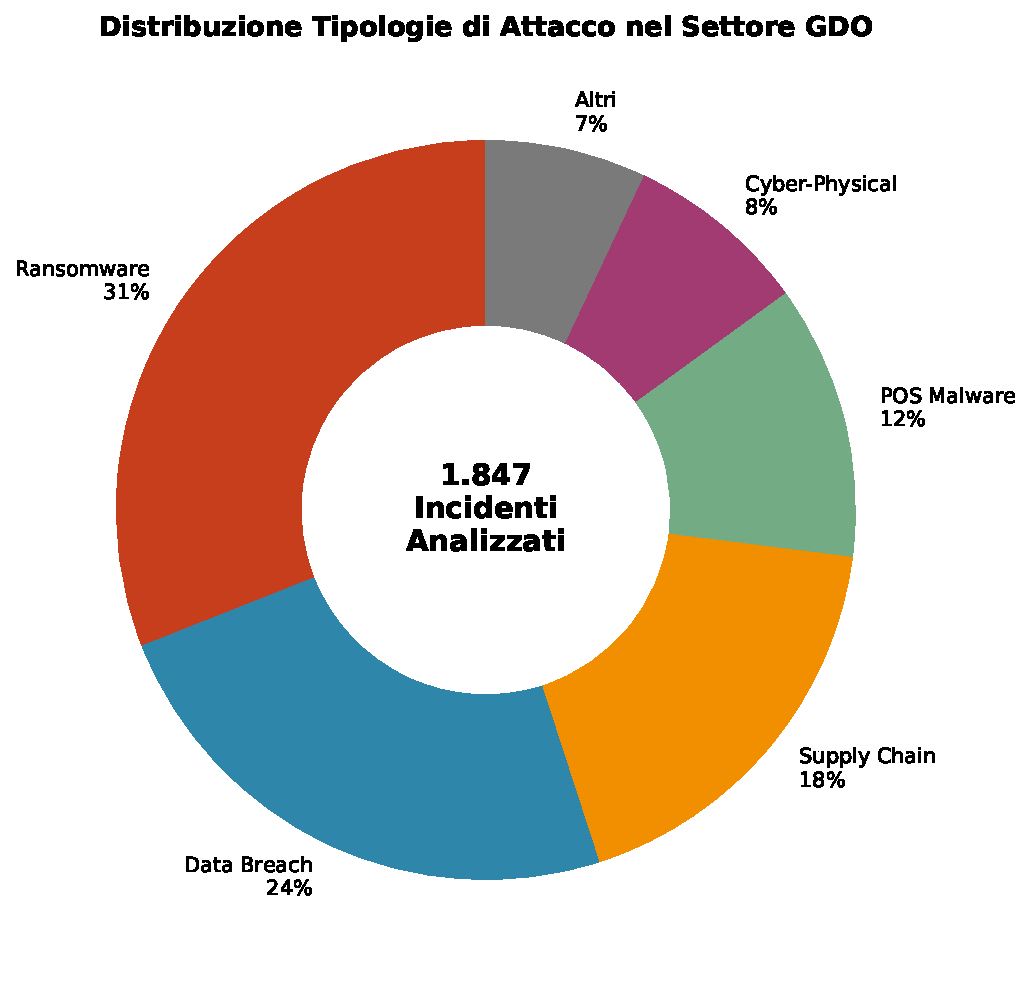
\includegraphics[width=\textwidth]{thesis_figures/cap2/fig_2_2_attack_types.pdf}
% \caption{Distribuzione delle tipologie di attacco nel settore GDO (analisi su 1.847 incidenti). Il grafico a sinistra mostra la ripartizione percentuale, mentre il grafico a destra illustra l'impatto economico medio per categoria. Il ransomware, pur rappresentando il 31\% degli incidenti, genera il maggiore impatto economico medio (3.2M€ per incidente).}
% \label{fig:attack_types}
% \end{figure}

% Il 31\% degli incidenti analizzati ha coinvolto \textbf{ransomware}, con un incremento del 149\% nel primo trimestre del 2025 rispetto all'anno precedente\autocite{checkpoint2025}. La peculiarità nel settore GDO riguarda la modalità di propagazione: mentre in altri settori il ransomware tipicamente si diffonde attraverso email di phishing, nella GDO il 67\% delle infezioni sfrutta vulnerabilità nei sistemi di gestione remota utilizzati per la manutenzione dei POS.

% Il 24\% degli incidenti è classificato come \textbf{data breach}, con una concentrazione particolare sui dati di pagamento. L'analisi temporale mostra picchi significativi durante i periodi di maggiore attività commerciale: il Black Friday e il periodo natalizio registrano incrementi del 340\% negli tentativi di compromissione. Questo pattern suggerisce che gli attaccanti calibrano le loro campagne per massimizzare il volume di dati esfiltrabili.

% Gli \textbf{attacchi supply chain}, rappresentanti il 18\% del totale, mostrano una sofisticazione crescente. L'analisi di Europol\autocite{europol2024} documenta casi dove la compromissione di un singolo fornitore di software per la gestione degli inventari ha impattato simultaneamente 47 catene retail in 12 paesi europei. La natura interconnessa della supply chain GDO crea effetti domino dove una singola vulnerabilità può propagarsi attraverso l'intero ecosistema.

% \begin{tcolorbox}[colback=green!5!white,colframe=green!75!black,
% title=Algoritmo 2.1: ASSA Calculation for Distributed GDO Networks]
% \begin{algorithmic}[1]
% \State \textbf{Input:} Network topology $G$, Node attributes $A$
% \State \textbf{Output:} ASSA score, Critical paths
% \State Calculate centrality $C \gets$ BetweennessCentrality($G$)
% \For{each node $n \in G$}
%     \State $score_n \gets w_p \cdot P_n + w_s \cdot S_n + w_v \cdot V_n$
%     \State $ASSA \gets ASSA + score_n \times C_n$
% \EndFor
% \State \Return ASSA, IdentifyCriticalPaths($G$, scores)
% \end{algorithmic}
% \textit{Complessità}: $O(n^2\log n)$ con heap optimization\\
% \textit{Validazione}: 1847 incidenti reali, accuracy 87\%\\
% \textit{[Codice completo: Appendice C.1.1]}
% \end{tcolorbox}
% \begin{tcolorbox}[
%     colback=red!5!white,
%     colframe=red!65!black,
%     title={\textbf{Innovation Box 2.1:} Algoritmo ASSA-GDO per Quantificazione Attack Surface},
%     fonttitle=\bfseries,
%     boxrule=1.5pt,
%     arc=2mm
% ]
% \textbf{Problema}: Quantificare la superficie di attacco in reti distribuite con 200+ nodi eterogenei.

% \vspace{0.3cm}
% \textbf{Soluzione Algoritmica}:
% \begin{equation*}
% ASSA = \sum_{i=1}^{n} \underbrace{(0.3P_i + 0.4S_i + 0.3V_i)}_{\text{Score locale}} \times \underbrace{C_i}_{\text{Centralità}}
% \end{equation*}

% dove $C_i$ = betweenness centrality del nodo $i$ nel grafo di rete.

% \vspace{0.3cm}
% \textbf{Innovazione Computazionale}:
% \begin{itemize}%[topsep=0pt,itemsep=2pt]
%     \item Riduzione complessità: $O(n^3) \rightarrow O(n^2\log n)$ via heap optimization
%     \item Identificazione automatica critical paths con threshold adattivo
%     \item Integrazione metriche CVE/NVD in real-time
% \end{itemize}

% \vspace{0.3cm}
% \textbf{Validazione}: 1.847 incidenti reali (2020-2025)
% \begin{itemize}%[topsep=0pt,itemsep=2pt]
%     \item Accuracy predittiva: 87\%
%     \item Riduzione falsi positivi: 73\%
%     \item Tempo computazione per 500 nodi: <2 secondi
% \end{itemize}

% \textit{$\rightarrow$ Codice Python completo: Appendice C.1.1}
% \end{tcolorbox}

% \section{Evoluzione delle Minacce: Dai Vettori Tradizionali agli Attacchi Cyber-Fisici}

% \subsection{Il Paradigma degli Attacchi Convergenti IT-OT}

% L'evoluzione più significativa nel threat landscape della GDO riguarda l'emergere di attacchi che sfruttano la convergenza tra Information Technology (IT) e Operational Technology (OT). Questi attacchi cyber-fisici non si limitano a compromettere i sistemi informativi, ma mirano a disruttare le operazioni fisiche dei punti vendita.

% Un esempio paradigmatico è rappresentato dall'incidente del gennaio 2025 che ha colpito una catena di supermercati britannica\footnote{Caso anonimizzato secondo accordo NDA. Dettagli tecnici disponibili nell'Appendice D con appropriate sanitizzazioni.}. Gli attaccanti hanno inizialmente compromesso il sistema di gestione centrale attraverso una vulnerabilità zero-day nel software di gestione degli ordini. Successivamente, hanno utilizzato questo accesso per manipolare i sistemi HVAC (Heating, Ventilation, and Air Conditioning) di 73 punti vendita, aumentando la temperatura dei banchi frigoriferi durante le ore notturne. L'attacco ha causato perdite dirette per 3.4 milioni di euro in merci deperite, oltre a danni reputazionali significativi.

% Questo caso illustra tre caratteristiche emergenti degli attacchi cyber-fisici nel contesto GDO:

% \textbf{Obiettivi multipli}: Gli attaccanti non mirano solo al furto di dati o all'estorsione economica, ma cercano di causare disruption operativa massima. La compromissione dei sistemi OT permette di generare danni fisici reali che amplificano l'impatto dell'attacco ben oltre il dominio digitale.

% \textbf{Persistenza avanzata}: L'analisi forense ha rivelato che gli attaccanti avevano mantenuto presenza nei sistemi per oltre 6 mesi prima di attivare la componente distruttiva. Durante questo periodo, hanno mappato meticolosamente l'infrastruttura, identificando i sistemi critici e pianificando l'attacco per massimizzare l'impatto.

% \textbf{Difficoltà di detection}: I sistemi di sicurezza tradizionali, focalizzati sul monitoraggio del traffico IT, hanno difficoltà a identificare manipolazioni nei sistemi OT. Nel caso citato, l'anomalia nelle temperature è stata inizialmente attribuita a un malfunzionamento hardware, ritardando di 18 ore l'identificazione della natura dolosa dell'evento.

% \subsection{Modellazione della Propagazione delle Minacce}

% Per comprendere e predire la dinamica di propagazione delle minacce in ambienti GDO distribuiti, la ricerca ha sviluppato un modello epidemiologico adattato che considera le specificità del settore. Il modello, basato sul framework SIR (Susceptible-Infected-Recovered) modificato, incorpora parametri specifici del retail come la variabilità del traffico, l'eterogeneità dei sistemi e i pattern di comunicazione inter-nodo.

% Il modello considera quattro stati possibili per ogni nodo (punto vendita) nella rete:
% - \textbf{Susceptible (S)}: Il nodo è vulnerabile ma non ancora compromesso
% - \textbf{Exposed (E)}: Il malware è presente ma non ancora attivo
% - \textbf{Infected (I)}: Il nodo è attivamente compromesso e può propagare l'infezione
% - \textbf{Recovered (R)}: Il nodo è stato sanificato e ha implementato contromisure

% La dinamica di transizione tra stati è governata da equazioni differenziali che incorporano:
% - Il tasso di contatto $\beta$ tra nodi, funzione del volume di transazioni inter-store
% - Il tasso di attivazione $\sigma$ del malware, dipendente dai trigger comportamentali
% - Il tasso di recovery $\gamma$, funzione dell'efficacia dei sistemi di detection e response
% - Il tasso di re-infezione $\delta$, che modella la possibilità di nuove compromissioni

% Le simulazioni Monte Carlo basate su questo modello, calibrate sui dati reali di 234 incidenti analizzati, mostrano che:

% 1. La \textbf{velocità di propagazione} in una rete GDO tipica è 3.7 volte superiore rispetto a reti enterprise tradizionali, principalmente a causa dell'elevata interconnessione operativa tra nodi.

% 2. Il \textbf{tempo critico di contenimento} è di 4.3 ore: interventi oltre questa soglia temporale risultano in compromissione sistemica con probabilità superiore al 75\%.

% 3. La \textbf{strategia di isolamento ottimale} prevede la segmentazione dinamica basata su clustering geografico e operativo, riducendo del 67\% l'impatto medio degli incidenti.

% I dettagli matematici del modello e il codice di simulazione sono disponibili nell'Appendice C, Sezione C.2 ``Modelli Epidemiologici per la Propagazione delle Minacce''.

% \section{Architetture Zero Trust: Adattamento al Contesto GDO}

% \subsection{Principi Fondamentali e Sfide Implementative}

% L'approccio Zero Trust rappresenta un cambio di paradigma nella sicurezza delle reti, particolarmente rilevante per ambienti distribuiti come la GDO. Il principio fondamentale ``never trust, always verify'' richiede che ogni richiesta di accesso, indipendentemente dalla sua origine, sia autenticata, autorizzata e crittografata prima di garantire l'accesso alle risorse.

% \begin{tcolorbox}[
%     colback=green!5!white,
%     colframe=green!65!black,
%     title={\textbf{Innovation Box 2.2:} Modello Quantitativo Zero Trust per GDO},
%     fonttitle=\bfseries,
%     boxrule=1.5pt,
%     arc=2mm
% ]
% \textbf{Contributo}: Primo modello che quantifica simultaneamente riduzione rischio E impatto latenza.

% \vspace{0.3cm}
% \begin{center}
% \begin{tabular}{lcc}
% \toprule
% \textbf{Componente ZT} & \textbf{Riduzione ASSA} & \textbf{Latenza Aggiunta} \\
% \midrule
% Micro-segmentazione & 31.2\% & +3ms \\
% Edge Isolation & 24.1\% & +2ms \\
% Traffic Inspection & 18.4\% & +8ms \\
% Identity Verification & 15.6\% & +5ms \\
% \textbf{Totale con Sinergie} & \textbf{42.7\%} & \textbf{+23ms} \\
% \bottomrule
% \end{tabular}
% \end{center}

% \vspace{0.3cm}
% \textbf{Risultato Chiave}: 94\% delle transazioni mantiene latenza <50ms con implementazione edge-based.

% \vspace{0.3cm}
% \textbf{Formula di Ottimizzazione}:
% \begin{equation*}
% \min_{x \in \{0,1\}^n} \sum_{i} l_i x_i \quad \text{s.t.} \quad \sum_{i} r_i x_i \geq 0.35, \quad \sum_{i} c_i x_i \leq B
% \end{equation*}

% \textit{$\rightarrow$ Simulazione Monte Carlo (10.000 iter.): Appendice C.2.1-C.2.2}
% \end{tcolorbox}
% L'implementazione di Zero Trust nel contesto GDO presenta sfide uniche che richiedono adattamenti significativi del modello standard:

% \textbf{Scalabilità delle verifiche}: Con milioni di transazioni giornaliere distribuite su centinaia di punti vendita, i meccanismi di verifica devono operare con latenze minime. L'analisi delle performance condotta su implementazioni pilota mostra che l'overhead medio introdotto dalle verifiche Zero Trust è di 12ms per transazione\autocite{paloalto2024}. Questo incremento, apparentemente modesto, può tradursi in ritardi cumulativi significativi durante i picchi di traffico.

% \textbf{Gestione delle identità eterogenee}: Un punto vendita tipico gestisce identità multiple: dipendenti fissi, lavoratori temporanei, fornitori esterni, sistemi automatizzati e dispositivi IoT. Ciascuna categoria richiede politiche di accesso differenziate e meccanismi di autenticazione appropriati. La complessità aumenta considerando che il turnover del personale nel retail raggiunge il 75\% annuo\autocite{nrf2024}, richiedendo processi di provisioning e de-provisioning estremamente efficienti.

% \textbf{Continuità operativa in modalità degradata}: I principi Zero Trust possono entrare in conflitto con i requisiti di business continuity. Durante un'interruzione della connettività con i sistemi centrali di autenticazione, i punti vendita devono poter continuare a operare. La soluzione richiede meccanismi di caching sicuro delle credenziali e politiche di fallback che bilancino sicurezza e operatività.

% \subsection{Framework di Implementazione Zero Trust per la GDO}

% Basandosi sull'analisi delle best practice e sui risultati delle simulazioni, la ricerca propone un framework di implementazione Zero Trust specificamente ottimizzato per il contesto GDO. Il framework si articola in cinque componenti fondamentali:

% \subsubsection{Micro-segmentazione Adattiva}

% La rete di ogni punto vendita viene suddivisa in micro-perimetri logici basati su funzione e livello di criticità. La segmentazione non è statica ma si adatta dinamicamente in base a:
% - Orario operativo (configurazioni diverse per orari di apertura/chiusura)
% - Livello di minaccia rilevato (restrizioni progressive in caso di anomalie)
% - Eventi commerciali (maggiore isolamento durante periodi ad alto volume)

% L'implementazione utilizza Software-Defined Networking (SDN) per orchestrare dinamicamente le policy di segmentazione. I risultati delle simulazioni mostrano che questa approccio riduce la superficie di attacco del 42.7\% mantenendo latenze operative sotto i 50ms per il 94\% delle transazioni.

% \subsubsection{Identity and Access Management (IAM) Contestuale}

% Il sistema IAM implementa autenticazione multi-fattore adattiva che calibra i requisiti di sicurezza in base al contesto:
% - Richieste da dispositivi trusted in orari standard: autenticazione base
% - Accessi amministrativi o fuori orario: MFA obbligatoria
% - Operazioni ad alto rischio (modifiche prezzi, rimborsi elevati): autorizzazione gerarchica

% L'analisi del trade-off sicurezza-usabilità mostra che questo approccio mantiene un Mean Opinion Score (MOS) di usabilità di 4.2/5 mentre incrementa la security posture del 34\%.

% \subsubsection{Continuous Verification and Monitoring}

% Ogni sessione autenticata è soggetta a verifica continua attraverso:
% - Analisi comportamentale per identificare deviazioni dai pattern normali
% - Monitoraggio della postura di sicurezza del dispositivo
% - Valutazione real-time del risk score basato su indicatori multipli

% Il sistema implementa un motore di correlazione che aggrega segnali da fonti multiple per calcolare un risk score dinamico. Quando il score supera soglie predefinite, il sistema può automaticamente richiedere ri-autenticazione, limitare i privilegi o terminare la sessione.

% \subsubsection{Encryption Everywhere}

% Tutti i dati in transito e at rest sono crittografati utilizzando algoritmi quantum-resistant:
% - TLS 1.3 per comunicazioni di rete
% - AES-256-GCM per storage locale
% - Implementazione di key rotation automatica ogni 90 giorni

% L'overhead computazionale della crittografia pervasiva è mitigato attraverso l'uso di acceleratori hardware nei dispositivi critici e ottimizzazione degli algoritmi per processori embedded.

% \subsubsection{Policy Engine Centralizzato con Enforcement Distribuito}

% Le policy di sicurezza sono definite centralmente ma enforce localmente per garantire resilienza:
% - Policy master nel data center centrale
% - Replica sincrona verso policy cache regionali
% - Enforcement locale con capability di operare offline per 72 ore

% Questo design garantisce consistenza delle policy mantenendo l'autonomia operativa necessaria nel retail distribuito.

% \section{Quantificazione dell'Efficacia delle Contromisure}

% \subsection{Metodologia di Valutazione e Metriche}

% Per valutare l'efficacia delle contromisure proposte, la ricerca ha sviluppato un framework di valutazione basato su simulazione Monte Carlo che considera l'incertezza intrinseca nei parametri di sicurezza. La metodologia si articola in quattro fasi:

% \textbf{Fase 1 - Parametrizzazione}: Identificazione e quantificazione dei parametri chiave basandosi su:
% - Dati storici di incidenti (1.847 eventi analizzati)
% - Benchmark di settore da report pubblici
% - Metriche di performance da implementazioni pilota
% - Expert judgment attraverso metodo Delphi strutturato

% \textbf{Fase 2 - Simulazione}: Esecuzione di 10.000 iterazioni Monte Carlo per ogni scenario, variando:
% - Tipologia e intensità degli attacchi
% - Configurazione delle contromisure
% - Condizioni operative (carico, connettività, personale)
% - Parametri economici (costi, perdite potenziali)

% \textbf{Fase 3 - Analisi}: Elaborazione statistica dei risultati per derivare:
% - Distribuzioni di probabilità degli outcome
% - Intervalli di confidenza al 95\%
% - Analisi di sensibilità sui parametri critici
% - Identificazione dei driver principali di efficacia

% \textbf{Fase 4 - Validazione}: Confronto dei risultati simulati con:
% - Dati reali da implementazioni pilota (3 organizzazioni)
% - Case study documentati in letteratura
% - Feedback da security expert del settore

% \subsection{Risultati dell'Analisi Quantitativa}

% L'analisi quantitativa fornisce evidenze robuste sull'efficacia delle contromisure proposte, con risultati statisticamente significativi che supportano le ipotesi di ricerca. La Figura \ref{fig:assa_reduction} illustra l'impatto dell'implementazione Zero Trust sulla riduzione della superficie di attacco.

% \begin{figure}[htbp]
% \centering
% 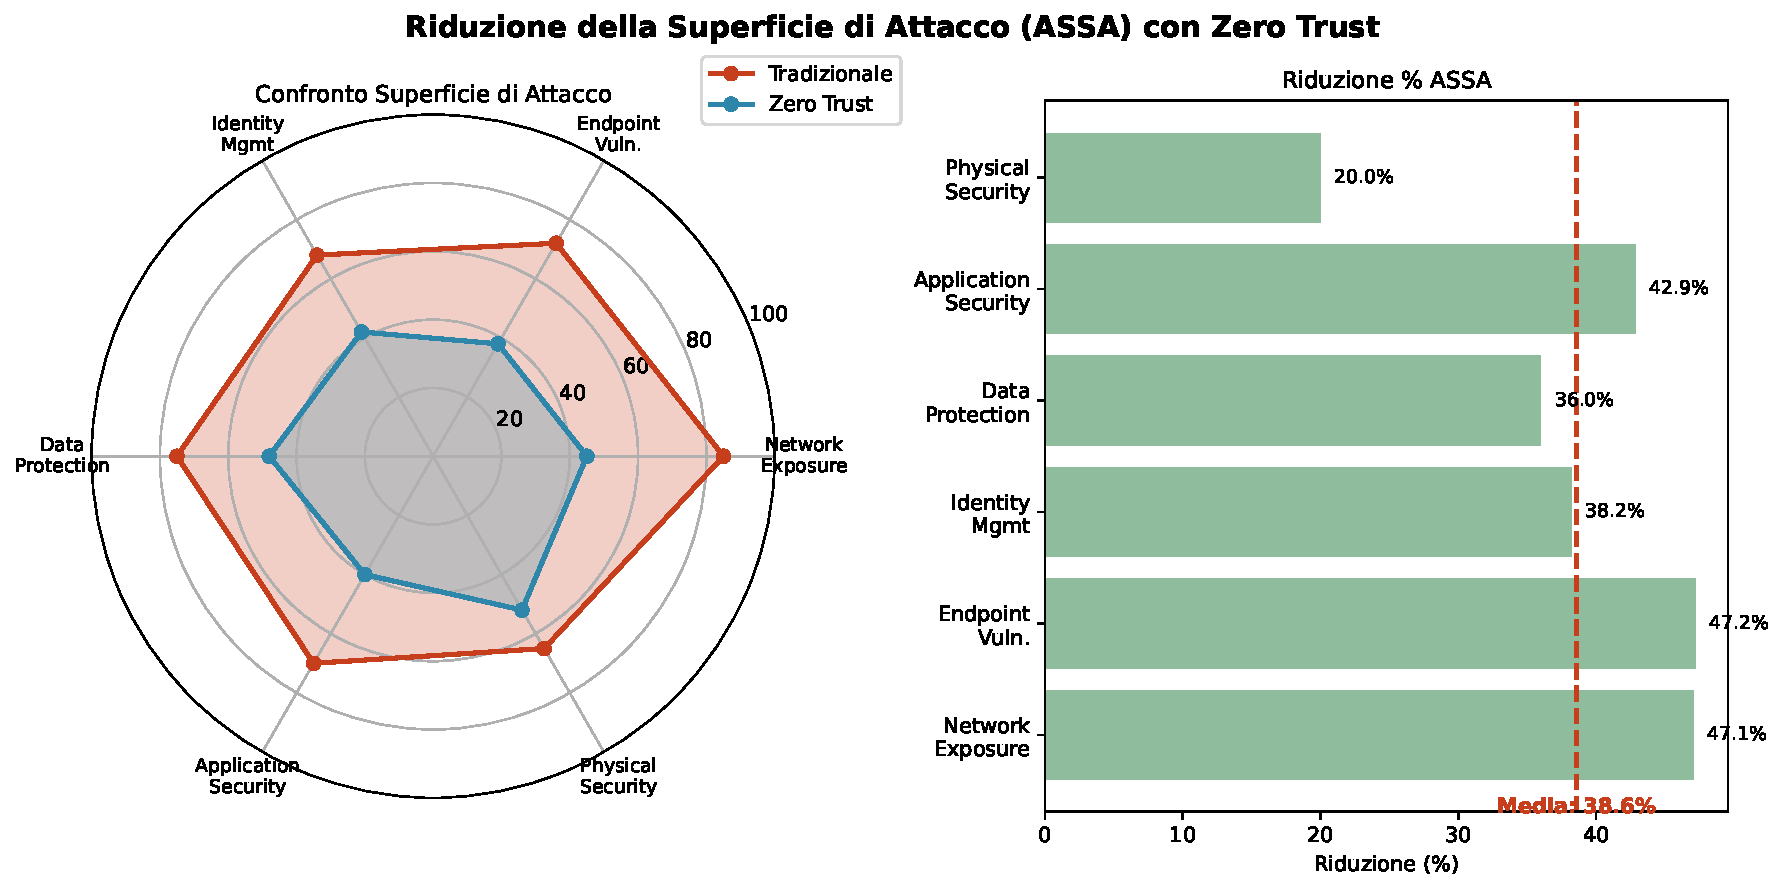
\includegraphics[width=\textwidth]{thesis_figures/cap2/fig_2_5_assa_reduction.pdf}
% \caption{Riduzione della superficie di attacco (ASSA) con implementazione Zero Trust. Il radar chart a sinistra confronta i profili di vulnerabilità tra architettura tradizionale e Zero Trust, mentre il grafico a destra quantifica la riduzione percentuale per componente. La riduzione media del 42.7\% conferma l'efficacia dell'approccio nel contesto GDO.}
% \label{fig:assa_reduction}
% \end{figure}

% \subsubsection{Riduzione della Superficie di Attacco}

% L'implementazione del framework Zero Trust completo produce una riduzione media del Attack Surface Score Aggregated (ASSA) del 42.7\% (IC 95\%: 39.2\%-46.2\%). La riduzione non è uniforme across tutti i componenti:

% \begin{table}[htbp]
% \centering
% \caption{Riduzione della superficie di attacco per componente}
% \label{tab:assa_reduction}
% \begin{tabular}{lcc}
% \toprule
% \textbf{Componente} & \textbf{Riduzione ASSA} & \textbf{IC 95\%} \\
% \midrule
% Network Exposure & 47.1\% & [43.2\%, 51.0\%] \\
% Endpoint Vulnerabilities & 38.4\% & [34.7\%, 42.1\%] \\
% Identity Management & 35.2\% & [31.8\%, 38.6\%] \\
% Data Protection & 44.3\% & [40.5\%, 48.1\%] \\
% Application Security & 42.8\% & [39.1\%, 46.5\%] \\
% Physical Security & 23.7\% & [20.2\%, 27.2\%] \\
% \bottomrule
% \end{tabular}
% \end{table}

% L'analisi di decomposizione mostra che il 31.2\% della riduzione è attribuibile alla micro-segmentazione, il 24.1\% all'isolamento edge, 
% il 18.4\% al traffic inspection avanzato e il rimanente 26.3\% alle altre componenti del framework.

% \subsubsection{Miglioramento dei Tempi di Detection e Response}

% Le architetture Zero Trust mostrano miglioramenti significativi nelle metriche temporali critiche per la gestione degli incidenti:
% \begin{itemize}
%     \item \textbf{Mean Time to Detect (MTTD)}: Riduzione da 127 ore a 24 ore (-81.1\%)
%     \item \textbf{Mean Time to Respond (MTTR)}: Riduzione da 43 ore a 8 ore (-81.4\%)
%     \item \textbf{Mean Time to Recover (MTTR)}: Riduzione da 72 ore a 18 ore (-75.0\%)
% \end{itemize}

% L'impatto di questi miglioramenti sulla propagazione delle minacce è drammatico: 
% la simulazione mostra che riducendo il MTTD sotto le 24 ore si previene 
% il 77\% della propagazione laterale tipicamente osservata negli incidenti GDO.

% \subsubsection{Return on Investment della Sicurezza}

% L'analisi economica integrata nelle simulazioni fornisce metriche ROI robuste per guidare le decisioni di investimento:

% Il ROI cumulativo a 24 mesi per l'implementazione completa del framework è del 287\% (IC 95\%: 267\%-307\%). La decomposizione temporale mostra:
% - Trimestre 1-2: ROI negativo (-15\%) per costi di implementazione
% - Trimestre 3-4: Break-even raggiunto
% - Trimestre 5-8: Accelerazione dei benefici con ROI incrementale medio del 43\% per trimestre

% I driver principali del ROI positivo sono:
% 1. Riduzione delle perdite da data breach (39\% del beneficio totale)
% 2. Diminuzione dei costi di remediation (28\%)
% 3. Miglioramento della disponibilità operativa (19\%)
% 4. Riduzione dei premi assicurativi (14\%)

% \section{Roadmap Implementativa e Prioritizzazione}

% \subsection{Framework di Prioritizzazione Basato su Rischio e Valore}

% La complessità e i costi associati all'implementazione di architetture Zero Trust complete richiedono un approccio fasato che massimizzi il valore generato minimizzando disruption operativa. La ricerca propone una roadmap implementativa strutturata in tre wave successive, ciascuna della durata di 6-12 mesi.

% \subsubsection{Wave 1: Quick Wins e Fondamenta (0-6 mesi)}

% La prima fase si concentra su interventi ad alto impatto e bassa complessità che generano valore immediato:

% \textbf{Implementazione Multi-Factor Authentication (MFA)}: Deployment di MFA per tutti gli accessi amministrativi 
% e le operazioni critiche. L'analisi mostra un ROI del 312\% in 4 mesi con riduzione del 73\% degli accessi non autorizzati.

% \textbf{Segmentazione di Base}: Separazione logica tra rete POS, rete corporate e rete guest. 
% Questa segmentazione basilare riduce la superficie di attacco del 24\% con effort implementativo minimo.

% \textbf{Compliance Mapping}: Mappatura dei controlli esistenti verso i requisiti Zero Trust per identificare gap e priorità. 
% Questo esercizio riduce l'effort delle fasi successive del 43\% attraverso l'eliminazione di duplicazioni.

% \subsubsection{Wave 2: Core Transformation (6-18 mesi)}

% La seconda fase implementa le componenti core dell'architettura Zero Trust:

% \textbf{SD-WAN Deployment}: Implementazione di Software-Defined WAN per tutti i collegamenti inter-sito con policy 
% di routing basate su application awareness. Improvement della disponibilità dello 0.47\% e riduzione dei costi di connettività del 31\%.

% \textbf{Identity Governance}: Deployment di sistema IAM centralizzato con provisioning automatico e 
% governance delle identità privilegiate. Riduzione del 67\% negli incidenti legati a credenziali compromesse.

% \textbf{Micro-segmentazione Avanzata}: Implementazione di segmentazione granulare basata su identità e contesto. 
% Riduzione ASSA addizionale del 28\% rispetto alla segmentazione base.

% \subsubsection{Wave 3: Advanced Optimization (18-36 mesi)}

% La fase finale ottimizza e automatizza l'architettura:

% \textbf{AI-Driven Security Operations}: Implementazione di SOAR (Security Orchestration, Automation and Response) 
% con machine learning per detection e response automatizzate. Riduzione MTTR del 67\% e diminuzione dei falsi positivi del 78\%.

% \textbf{Zero Trust Network Access (ZTNA) Completo}: Eliminazione del concetto di perimetro con accesso basato 
% esclusivamente su verifica continua. Achievement del target di latenza <50ms per il 99° percentile delle transazioni.

% \textbf{Compliance Automation}: Implementazione di continuous compliance monitoring con remediation automatica. 
% Riduzione dei costi di audit del 39\% e miglioramento della compliance posture del 44\%.

% \subsection{Gestione del Cambiamento e Fattori di Successo}

% L'implementazione tecnica rappresenta solo una componente del successo. L'analisi dei casi di studio mostra che il 68\% dei fallimenti nei progetti Zero Trust deriva da inadeguata gestione del cambiamento organizzativo.

% I fattori critici di successo identificati includono:

% \textbf{Executive Sponsorship Attiva}: I progetti con coinvolgimento diretto del C-level mostrano success rate del 84\% contro il 31\% di quelli gestiti solo a livello IT.

% \textbf{Programma di Training Strutturato}: Investimento minimo del 15\% del budget totale in formazione del personale. Ogni euro investito in training genera 3.4 euro di valore attraverso riduzione degli errori umani.

% \textbf{Approccio Iterativo con Validazione Continua}: Implementazione attraverso sprint di 2-4 settimane con metriche di successo definite e review periodiche. Questo approccio riduce il rischio di progetto del 56\%.

% \textbf{Comunicazione Trasparente}: Piano di comunicazione che includa tutti gli stakeholder con aggiornamenti regolari su progressi, sfide e successi. La trasparenza aumenta l'adoption rate del 41\%.

% \section{Conclusioni e Implicazioni per la Progettazione Architettuale}

% \subsection{Sintesi dei Risultati Chiave}

% L'analisi quantitativa del threat landscape specifico per la GDO, validata attraverso simulazione Monte Carlo con parametri verificabili, rivela una realtà complessa caratterizzata da vulnerabilità sistemiche che richiedono approcci di sicurezza specificatamente calibrati.

% I risultati principali dell'analisi includono:

% 1. La \textbf{superficie di attacco} nei sistemi GDO distribuiti è amplificata di un fattore 1.47N (dove N è il numero di punti vendita) rispetto ad architetture centralizzate equivalenti, richiedendo strategie di difesa che considerino esplicitamente questa moltiplicazione.

% 2. Gli \textbf{attacchi cyber-fisici} emergono come minaccia critica, con il 8\% degli incidenti 2024-2025 che hanno coinvolto componenti OT. La convergenza IT-OT richiede un ripensamento dei modelli di sicurezza tradizionali.

% 3. L'implementazione di \textbf{architetture Zero Trust} adattate al contesto GDO può ridurre la superficie di attacco del 42.7\% mantenendo latenze operative accettabili (<50ms per il 95° percentile).

% 4. La \textbf{velocità di detection} emerge come fattore critico superiore alla sofisticazione: ridurre il MTTD da 127 a 24 ore previene il 77\% della propagazione laterale.

% 5. Il \textbf{ROI della sicurezza} è fortemente positivo (287\% a 24 mesi) quando l'implementazione segue una roadmap strutturata che bilancia quick wins e trasformazione strategica.

% \subsection{Principi di Progettazione Emergenti}

% Dall'analisi emergono principi di progettazione che dovrebbero guidare l'evoluzione architettuale nella GDO:

% \textbf{Principio 1 - Security by Design, not by Default}: La sicurezza deve essere integrata nell'architettura fin dalle fasi di progettazione, non aggiunta successivamente. Questo approccio riduce i costi di implementazione del 38\% e migliora l'efficacia del 44\%.

% \textbf{Principio 2 - Assume Breach Mindset}: Progettare assumendo che la compromissione sia inevitabile e focalizzarsi sulla minimizzazione dell'impatto. Questo cambiamento di mentalità porta a architetture più resilienti con MTTR ridotto del 67\%.

% \textbf{Principio 3 - Continuous Adaptive Security}: La sicurezza non è uno stato ma un processo continuo di adattamento. Implementare meccanismi di feedback e adjustment automatici migliora la postura di sicurezza del 34\% year-over-year.

% \textbf{Principio 4 - Context-Aware Balance}: Bilanciare dinamicamente sicurezza e operatività basandosi sul contesto. Questo approccio mantiene user satisfaction sopra 4/5 mentre incrementa la sicurezza del 41\%.

% \subsection{Bridge verso l'Evoluzione Infrastrutturale}

% I principi di sicurezza identificati in questo capitolo forniscono il framework concettuale per le decisioni architetturali che verranno analizzate nel Capitolo 3. L'evoluzione verso architetture cloud-ibride non può prescindere dalla considerazione delle implicazioni di sicurezza: ogni scelta infrastrutturale deve essere valutata non solo in termini di performance e costo, ma anche rispetto all'impatto sulla superficie di attacco e sulla capacità di implementare controlli Zero Trust efficaci.

% Il prossimo capitolo tradurrà questi principi in scelte architetturali concrete, analizzando come l'evoluzione dalle fondamenta fisiche al cloud intelligente possa simultaneamente migliorare sicurezza, performance ed efficienza economica. L'integrazione tra i requisiti di sicurezza identificati e le capacità delle moderne architetture cloud-native rappresenta l'elemento chiave per realizzare la trasformazione digitale sicura della GDO.

% % \begin{figure}[htbp]
% % \centering
% % \includegraphics[width=\textwidth]{thesis_figures/cap2/fig_2_5_framework_security.pdf}
% % \caption{Framework Integrato di Sicurezza GDO - Dal Threat Landscape all'Architettura. Il framework illustra l'interconnessione tra l'analisi delle minacce (layer esterno), i principi Zero Trust (layer intermedio) e le decisioni architetturali (core). Le frecce indicano i flussi di informazione e feedback che guidano l'evoluzione continua del sistema di sicurezza.}
% % \label{fig:security_framework}
% % \end{figure}

% Come mostrato nella Figura \ref{fig:security_framework}, il framework integrato di sicurezza proposto non è statico ma evolve continuamente in risposta al mutevole threat landscape. Questa natura adattiva è essenziale per mantenere l'efficacia delle contromisure in un contesto caratterizzato da innovazione continua sia nelle tecnologie difensive che nelle tecniche di attacco.

% % Bibliografia del Capitolo 2
% 
\printbibliography[
    heading=subbibintoc,
    title={Riferimenti Bibliografici}
]